\chapter{\IfLanguageName{dutch}{Stand van zaken}{State of the art}}%
\label{ch:stand-van-zaken}

% Tip: Begin elk hoofdstuk met een paragraaf inleiding die beschrijft hoe
% dit hoofdstuk past binnen het geheel van de bachelorproef. Geef in het
% bijzonder aan wat de link is met het vorige en volgende hoofdstuk.

% Pas na deze inleidende paragraaf komt de eerste sectiehoofding.

% Dit hoofdstuk bevat je literatuurstudie. De inhoud gaat verder op de inleiding, maar zal het onderwerp van de bachelorproef *diepgaand* uitspitten. De bedoeling is dat de lezer na lezing van dit hoofdstuk helemaal op de hoogte is van de huidige stand van zaken (state-of-the-art) in het onderzoeksdomein. Iemand die niet vertrouwd is met het onderwerp, weet nu voldoende om de rest van het verhaal te kunnen volgen, zonder dat die er nog andere informatie moet over opzoeken \autocite{Pollefliet2011}.

% Je verwijst bij elke bewering die je doet, vakterm die je introduceert, enz.\ naar je bronnen. In \LaTeX{} kan dat met het commando \texttt{$\backslash${textcite\{\}}} of \texttt{$\backslash${autocite\{\}}}. Als argument van het commando geef je de ``sleutel'' van een ``record'' in een bibliografische databank in het Bib\LaTeX{}-formaat (een tekstbestand). Als je expliciet naar de auteur verwijst in de zin (narratieve referentie), gebruik je \texttt{$\backslash${}textcite\{\}}. Soms is de auteursnaam niet expliciet een onderdeel van de zin, dan gebruik je \texttt{$\backslash${}autocite\{\}} (referentie tussen haakjes). Dit gebruik je bv.~bij een citaat, of om in het bijschrift van een overgenomen afbeelding, broncode, tabel, enz. te verwijzen naar de bron. In de volgende paragraaf een voorbeeld van elk.

% \textcite{Knuth1998} schreef een van de standaardwerken over sorteer- en zoekalgoritmen. Experten zijn het erover eens dat cloud computing een interessante opportuniteit vormen, zowel voor gebruikers als voor dienstverleners op vlak van informatietechnologie\cite{Creeger2009}.

% Let er ook op: het \texttt{cite}-commando voor de punt, dus binnen de zin. Je verwijst meteen naar een bron in de eerste zin die erop gebaseerd is, dus niet pas op het einde van een paragraaf.

Voor er een vergelijking kan gemaakt worden tussen monolithische en microservices architectuur moeten we eerst eens terug kijken naar hoe deze twee architecturen zich tot elkaar verhouden.


\section{Monolithische architectuur}
Laten we beginnen met monolithische applicaties. Hoewel ze enkele voordelen bieden, worden ze vaak geconfronteerd met aanzienlijke nadelen die van invloed kunnen zijn op de ontwikkeling, schaalbaarheid en onderhoud van de software.


Een van de belangrijkste nadelen is de groeiende complexiteit van de codebase naarmate de applicatie evolueert. Deze toenemende complexiteit kan leiden tot overbelasting van de ontwikkelomgeving, waardoor de productiviteit van ontwikkelaars afneemt. Het veranderen van de technologiestack van de applicatie kan een uitdagende taak zijn en het herstructureren van de codebase wordt bemoeilijkt door de onvoorspelbare impact op de applicatiefunctionaliteit.


Een kritiek punt is het risico van volledige uitval wanneer een enkele functie of component van de applicatie faalt. Dit kan leiden tot aanzienlijke downtime en verstoring van de dienstverlening, wat zowel de gebruikerservaring als de bedrijfsactiviteiten negatief kan beïnvloeden. Bovendien neemt de kwaliteit van een monolithische architectuur geleidelijk af in de loop van de tijd door de constante toevoeging van nieuwe componenten, wat resulteert in een afname van de verwerkingssnelheid.


De architectuur wordt ook als veeleisend ervaren om te begrijpen, vooral naarmate de codebase groeit. Dit vereist meestal een diepgaande kennis van het gehele systeem, en zelfs ervaren ontwikkelaars kunnen moeite hebben om de complexiteit te doorgronden. Nieuwe ontwikkelaars hebben vaak een langere inwerkperiode nodig om zich vertrouwd te maken met de codebase en effectief bij te dragen aan de ontwikkeling van de applicatie.


Schaalbaarheidsproblemen vormen ook een uitdaging bij monolithische architecturen. Omdat alle componenten binnen dezelfde codebase worden uitgevoerd, kan het moeilijk zijn om specifieke delen van de applicatie te schalen zonder de algehele prestaties te beïnvloeden. Dit kan leiden tot inefficiënt gebruik van middelen en beperkingen in de mogelijkheid om snel te reageren op veranderende gebruikersbehoeften.


Ondanks deze nadelen hebben monolithische applicaties ook enkele voordelen. Ze zijn over het algemeen eenvoudiger te ontwikkelen, te implementeren en te beheren, vooral voor kleine tot middelgrote projecten met beperkte complexiteit. Bovendien zijn ze gemakkelijker te debuggen omdat alle functionaliteit binnen dezelfde codebase wordt uitgevoerd, wat het opsporen en oplossen van fouten vereenvoudigt.


Het is belangrijk om deze voordelen af te wegen tegen de nadelen en om de juiste architectuurkeuze te maken op basis van de specifieke behoeften en vereisten van het project.\autocite{Alexandra2022}.

\begin{figure}[H]
	\centering	
	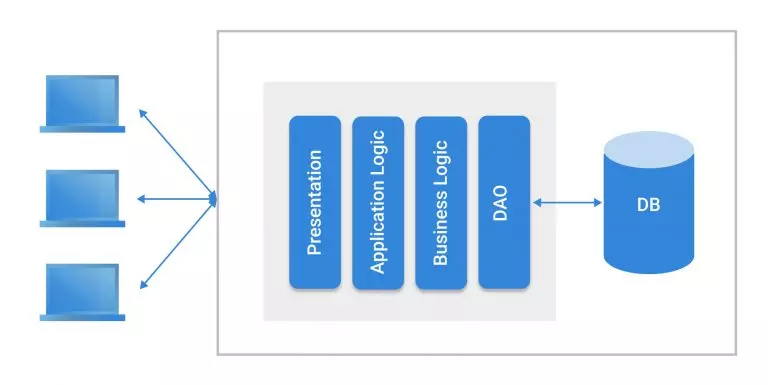
\includegraphics[width = 18cm]{MonolithicImage1.png} 
	\caption{Monoliet} 
	\label{fig:MonolietBP} 
\end{figure}
\FloatBarrier

\section{Microservices architectuur}
Dan hebben we microservices architecturen die een manier zijn  om grote softwareprojecten op te splitsen in losjes gekoppelde modules, die met elkaar communiceren via eenvoudige Application Programming Interfaces (API's). Volgens Adrian Cockcroft, voorheen werkzaam bij Netflix, is "Een microservices-architectuur een servicegerichte architectuur, samengesteld uit losjes gekoppelde elementen met begrensde contexten " (vertaald vanuit het Engels) \cite{Richardson2018}.

Microservices bieden diverse voordelen die gericht zijn op flexibiliteit, schaalbaarheid en foutisolatie. Eén van de belangrijkste voordelen is de mogelijkheid om onafhankelijke, herbruikbare componenten te creëren. Deze componenten kunnen afzonderlijk worden geïmplementeerd in andere applicaties zonder invloed op andere eenheden. Het modulaire karakter van microservices maakt het eenvoudig te debuggen, schalen en begrijpen, wat bijdraagt aan een snellere ontwikkeling en implementatie. 
Microservices stellen ontwikkelaars in staat om specifieke componenten te schalen of ongewijzigd te laten, waardoor een hoog niveau van flexibiliteit ontstaat. Verbeterde foutisolatie is ook een voordeel, omdat falen in één module de prestaties van de gehele applicatie niet significant beïnvloedt. Daarnaast biedt de mogelijkheid om nieuwe technologieën toe te voegen en te testen, evenals het elimineren van leverancier- of technologielock-in, extra voordelen voor wendbaarheid en innovatie. 

Aan de andere kant zijn er ook nadelen verbonden aan microservices. De architectuur kan te ingewikkeld worden naarmate het systeem groeit, waardoor het beheer bemoeilijkt wordt. Het testen kan veeleisend zijn, vooral bij complexe systemen en het onderhoud kan duurder worden naarmate meer eenheden worden toegevoegd. Beveiligingsproblemen zijn een zorg, aangezien de gedistribueerde aard van microservices verschillende faalpunten introduceert. 
De complexiteit van communicatie tussen services, de kosten van individuele servers en databases voor elke microservice en de kwetsbaarheid voor beveiligingsproblemen zijn belangrijke nadelen. Ook brengt de complexiteit van coördinatie tussen services uitdagingen met zich mee bij implementatie, vooral voor kleine bedrijven die snel willen creëren en itereren. Het testen van microservices-gebaseerde applicaties kan omslachtig zijn en het opsporen van fouten vereist grondig doorzoeken van de logboeken van elke service. 
Hoewel microservices veel voordelen bieden, moeten organisaties zorgvuldig afwegen of de voordelen opwegen tegen de complexiteit en uitdagingen die de implementatie van deze architectuur met zich meebrengt.

\begin{figure}[H]
	\centering	
	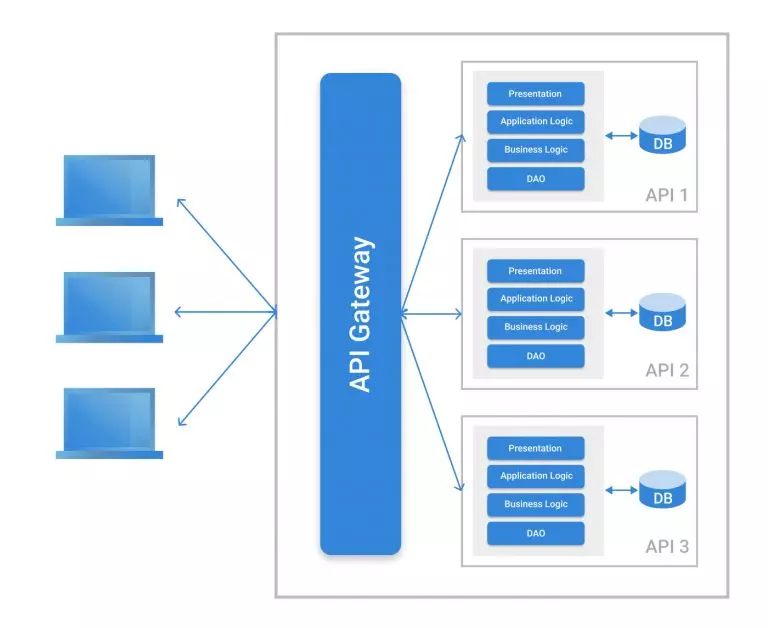
\includegraphics[width = 12cm]{MicroserviceImage1.png} 
	\caption{Microservice} 
	\label{fig:MicroserviceBP} 
\end{figure}
\FloatBarrier

\section{Lehman's wetten van software-evolutie}
Al lang voor het ontstaan van microservice kwam Lehman met zijn acht wetten van software-evolutie. Deze wetten beschrijven de dynamiek van softwaresystemen over tijd en benadrukken de noodzaak van voortdurende aanpassing aan nieuwe behoeften, beheersing van toenemende complexiteit en behoud van stabiliteit en bekendheid. Het behoud van organisatorische stabiliteit en bekendheid, gecombineerd met voortdurende groei in functionaliteit, vormt de kern van Lehman's inzichten. Tevens waarschuwen de wetten voor mogelijke afname in kwaliteit over tijd, waarbij een feedbacksysteem cruciaal is voor een succesvolle evolutie, met erkenning van de rol van gebruikersfeedback in het stimuleren van toekomstige ontwikkelingen \autocite{Richardson}.

Het valideren van software-architectuur tegen de wetten van Lehman helpt ervoor te zorgen dat het systeem robuust, aanpasbaar en onderhoudbaar is gedurende zijn levensduur. Het stelt architecten in staat om op uitdagingen te anticiperen en oplossingen te ontwerpen die op elegante wijze de onvermijdelijke veranderingen en complexiteiten van software-evolutie kunnen opvangen. Deze validatie leidt tot betere softwarekwaliteit, verbeterde gebruikerstevredenheid en duurzamere ontwikkelpraktijken.


\begin{enumerate}
	\item \textbf{Continuing Change:} Lehman stelt dat een softwaresysteem in de loop der tijd steeds minder bevredigend wordt voor gebruikers, tenzij het voortdurend wordt aangepast aan nieuwe behoeften. De noodzaak van voortdurende aanpassing staat hierbij centraal.
	
	\item \textbf{Increasing Complexity:} Softwaresystemen worden volgens Lehman steeds complexer, tenzij actieve inspanningen worden geleverd om deze complexiteit te verminderen. Deze wet benadrukt de essentie van proactieve maatregelen om de inherente neiging tot complexiteitsgroei te beheersen.
	
	\item \textbf{Self-Regulation:} Het proces van software-evolutie reguleert volgens Lehman zichzelf, met een distributie van product- en procesartefacten die dicht bij normaal ligt. Dit impliceert een natuurlijk evenwicht in het evolutieproces, in lijn met typische statistische patronen.
	
	\item \textbf{Conservation of Organizational Stability:} Het gemiddelde effectieve wereldwijde activiteitsniveau op een evoluerend softwaresysteem verandert niet in de loop der tijd. Dit suggereert dat de hoeveelheid werk in elke release volgens Lehman relatief constant blijft en bijdraagt aan de stabiliteit van het ontwikkelingsproces.
	
	\item \textbf{Conservation of Familiarity:} De hoeveelheid nieuwe inhoud in opeenvolgende releases neigt constant te blijven of af te nemen. Deze wet belicht de trend om het behoud of de vermindering van de introductie van nieuwe elementen in software-releases.
	
	\item \textbf{Continuing Growth:} De hoeveelheid functionaliteit in een softwaresysteem zal toenemen om aan de verwachtingen van gebruikers te voldoen. Dit erkent de noodzaak om de mogelijkheden van software te verbeteren voor voortdurende relevantie en bruikbaarheid.
	
	\item \textbf{Declining Quality:} Een softwaresysteem wordt gezien als afnemend in kwaliteit, tenzij het ontwerp zorgvuldig wordt onderhouden en aangepast aan nieuwe operationele beperkingen. Dit onderstreept het belang van continue kwaliteitsborging en ontwerpoverwegingen.
	
	\item \textbf{Feedback System:} Het succesvol evolueren van een softwaresysteem vereist erkenning van het ontwikkelingsproces als een multi-loop, multi-agent, multi-level feedbacksysteem. Naarmate een softwaresysteem ouder wordt, wordt het steeds moeilijker te veranderen vanwege de complexiteit van zowel artefacten als processen, waarbij de rol van gebruikersfeedback in de toekomstige evolutie wordt erkend. \autocite{Godfrey2013}
\end{enumerate}

\section{Ontstaan van microservices}
Microservices zijn ontstaan uit frustraties met traditionele monolithische architectuur. Deze benadering omvat het bouwen van applicaties als suites van onafhankelijke, schaalbare services. Elke service heeft een duidelijke modulegrens, waardoor ze zelfs in verschillende programmeertalen kunnen worden geschreven en door verschillende teams kunnen worden beheerd. De microservices-stijl is niets nieuws. De oorsprong gaat terug tot Unix-ontwerpprincipes. Hoewel er geen formele definitie bestaat, delen microservice-architecturen gemeenschappelijke kenmerken die bijdragen aan hun flexibiliteit en schaalbaarheid. \autocite{Fowler2014}.

\begin{enumerate}
	\item \textbf{Componentization via Services:} Microservices worden behandeld als onafhankelijke componenten die afzonderlijk kunnen worden geïmplementeerd en bijgewerkt.
	
	\item \textbf{Organized around Business Capabilities:} Microservices zijn georganiseerd rond zakelijke mogelijkheden, wat betekent dat elke service overeenkomt met een zakelijke functionaliteit.
	
	\item \textbf{Products not Projects:} teams bezitten een bepaald product gedurende de volledige levensduur ervan, in plaats van alleen maar aan projecten te werken.
	
	\item \textbf{Smart endpoints and dumb pipes:} Applicaties die zijn opgebouwd uit microservices streven ernaar zo ontkoppeld en samenhangend mogelijk te zijn. Ze communiceren met elkaar via eenvoudige API’s, terwijl ze de onderliggende communicatie-complexiteit weghouden van de services. 
	
	\item \textbf{Decentralized Governance:} Verschillende diensten kunnen verschillende technologieën gebruiken (programmeertalen, databases, enz.). Er is geen gestandaardiseerd mandaat voor alle diensten.
	
	\item \textbf{Decentralized Data Management:} Elke dienst heeft zijn eigen database om de ontkoppeling van andere diensten te garanderen.
	
	\item \textbf{Infrastructure Automation:} gebruik van continue integratie en continue implementatie om de services te beheren.
	
	\item \textbf{Design for failure:} Diensten moeten worden ontworpen met het oog op het feit dat ze zullen mislukken. Dit helpt bij het bouwen van veerkrachtige systemen.
	
	\item \textbf{Evolutionary Design:} Het is de bedoeling dat het systeemontwerp in de loop van de tijd evolueert en nieuwe technologieën en praktijken kunnen worden toegepast wanneer dat nodig is. \autocite{Fowler2014}.
\end{enumerate}

\section{Servicemeshes}
Deze adoptie van microservices architectuur heeft geleid tot de opkomst van servicemeshes als een mechanisme voor het beheren van de communicatie en interactie tussen de verschillende services binnen een applicatie. Een servicemesh is een abstractielaag die een reeks functies biedt, zoals load balancing, service discovery, monitoring en beveiliging, die essentieel zijn voor het schalen en beheren van microservices.


Een belangrijke architecturale overweging bij het gebruik van een servicemesh is service discovery. In tegenstelling tot een monolithische architectuur, waarbij functionaliteiten vaak hardgecodeerde afhankelijkheden hebben, maakt een servicemesh gebruik van dynamische service discovery. Dit stelt services in staat om automatisch nieuwe services te ontdekken en ermee te communiceren zonder handmatige configuratiewijzigingen. Een voorbeeld van een servicemesh implementatie die service discovery mogelijk maakt, is Istio
 \autocite{Morgan2021}.

Een andere belangrijke aspect is load balancing. Een servicemesh verdeelt het verkeer gelijkmatig over de beschikbare service instances, waardoor de prestaties worden geoptimaliseerd, de belasting op afzonderlijke instances onder controle blijft en er ad hoc extra instances kunnen opgespind worden. Dit is vooral nuttig in bedrijfsapplicaties waar veel services parallel moeten worden geschaald om aan de vraag te voldoen\autocite{Ciobotaru2020}.

Monitoring en tracing van service traffic zijn ook cruciale aspecten bij het gebruik van een servicemesh. Door het instrumenteren van services met monitoring- en tracingfunctionaliteit, kan een servicemesh gedetailleerd inzicht bieden in de prestaties en het gedrag van services. Dit is met name waardevol in bedrijfsapplicaties waar de complexiteit van de interacties tussen services kan leiden tot moeilijkheden bij het identificeren en oplossen van problemen. Servicemeshes verhogen de weerbaarheid door het implementeren van verschillende resilience patterns. Hierdoor kan tijdelijke onbeschikbaarheid of overbelasting van services opgevangen worden\autocite{Ciobotaru2021}.

Naast deze technische aspecten spelen ook operationele overwegingen een rol bij het gebruik van een servicemesh. Het implementeren en beheren van een servicemesh kan complex zijn en vereist vaak een zorgvuldige planning en configuratie. Bovendien brengt het gebruik van een servicemesh extra overhead met zich mee, zowel in termen van resourceverbruik als in operationele complexiteit. Het is daarom belangrijk om de voordelen van een servicemesh af te wegen tegen de extra kosten en complexiteit die ermee gepaard gaan, vooral voor kleinere applicaties met beperkte resources.


Al met al biedt het gebruik van een servicemesh aanzienlijke voordelen voor het beheren van microservices architectuur, maar het is belangrijk om zowel de technische als operationele aspecten zorgvuldig te overwegen voordat tot implementatie wordt overgegaan.


\section{Kort samengevat}

Een monolithische architectuur biedt eenvoud en een eenvoudige implementatie, maar kan uitdagend zijn bij groei. Microservices bieden flexibiliteit en schaalbaarheid, maar kunnen complexer en duurder zijn in onderhoud.

Een monolithische architectuur bestaat uit één codebase met alle functionaliteit, terwijl een microservices architectuur gebruik maakt van onafhankelijke services. Microservices bieden flexibiliteit en schaalbaarheid, maar brengen ook complexiteit met zich mee, zoals service discovery en monitoring. De juiste architectuurkeuze hangt af van de behoeften en complexiteit van het project.

Lehman's acht wetten van software-evolutie schetsen de dynamiek van softwaresystemen in de loop van de tijd. Ze onderstrepen de noodzaak van voortdurende aanpassing aan nieuwe behoeften, het beheersen van toenemende complexiteit, en het handhaven van evenwicht in het evolutieproces. Het behoud van organisatorische stabiliteit en vertrouwdheid, tezamen met voortdurende groei in functionaliteit, vormt de kern van Lehman's inzichten. Tegelijkertijd waarschuwen de wetten voor mogelijke afname in kwaliteit na verloop van tijd, waarbij een feedbacksysteem cruciaal is voor een succesvolle evolutie, met erkenning van de rol van gebruikersfeedback in het stimuleren van toekomstige ontwikkelingen. 

Lehman's wetten vinden dus toepassing in zowel monolithische als gedistribueerde (microservices) systemen. In het geval van monolithische architecturen benadrukken deze wetten de noodzaak van voortdurende aanpassing aan veranderende eisen, beheersing van complexiteit en behoud van stabiliteit en bekendheid. 

De vraag rijst echter of microservices een oplossing kunnen bieden voor enkele uitdagingen die voortvloeien uit Lehman's wetten.

